\section{Röntgenstrahlung}
Die Entdeckung der Röntgenstrahlung gelang Wilhelm Conrad Röntgen 1895 durch Beobachtungen von Fluoreszenzeffekten an Bariumplatincyanür in der Nähe einer Elektronenröhre (org.: \textit{Hittorf'sche Vacuumröhre}). Diese war eigentlich mit einem schwarzen Karton ummantelt und die im inneren entstehende Strahlung sollte dadurch nach bisherigem Kenntnisstand abgeschirmt sein. Damals vermutete Röntgen, dass die von ihm entdeckten X-Strahlen longitudinale Schwingungen aus dem Äther seien \cite[Absätze~1,2,17]{wcrpaper}. Heute wissen wir, dass es sich bei Röntgenstrahlen um transversale, elektromagnetische Strahlung in einem Energiebereich von etwa \SI{15}{\electronvolt} bis zu etwa \SI{1.2}{\mega\electronvolt} handelt, wobei die Grenzen zwischen UV- und Röntgenstrahlung im unteren Energiebereich bei etwa \SI{10}{\electronvolt} bis \SI{500}{\electronvolt}  und zwischen Röntgen- und Gammastrahlung im oberen Energiebereich um ca. \SI{500}{\kilo\electronvolt} nicht fest definiert sind.\newline

\begin{figure}[H] %h:Grafik an dieser Stelle einbinden. Falls das nicht geht: %t:oben auf der Seite. Wenn dies auch nicht möglich ist: %b:am Fuß der Seite oder %p:auf der nächsten Seite %! is specified, then ignore the restrictions of placing floating objects %H (float package) forces position
  \centering
     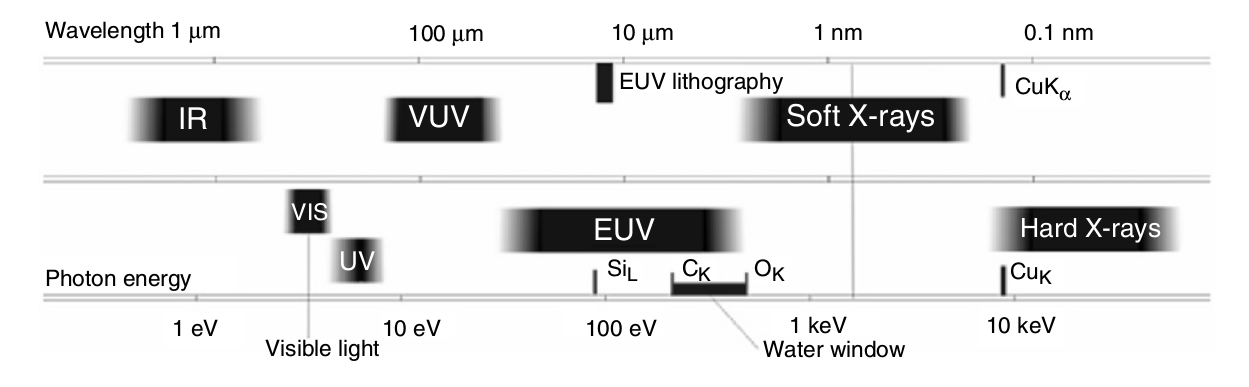
\includegraphics[width=0.9\textwidth]{illustrations/spectrumEMradiation.png}
  \caption[Spektrum EM-Strahlung]{Darstellung des Spektrums elektromagnetischer Strahlung von infrarotem(IR), über sichtbares(VIS) und ultraviolettem(UV) Licht bis zu Röntgenstrahlung. Außerdem sind die Abstufungen des UV Lichts in vacuum(VUV) und extrem(EUV), weiche und harte Röntgenstrahlung und das Wasserfenster dargestellt. \cite[S.~34]{bbbook}}
  \label{fig:spectrumEMradiation}
\end{figure}

\noindent Die Erzeugung von Röntgenstrahlen kann auf 2 Arten geschehen: Einerseits entsteht durch das Ablenken von Elektronen die sog. "Bremsstrahlung"\,\,(\cref{fig:spectrumXray}) welche zu einem kontinuierlichen Spektrum führt und die Röntgen wohl ursprünglich indirekt beobachtet hat. Andererseits liefern Schalenübergänge von Elektronen ein sog. charakteristisches Röntgenspektrum welches sich eindeutig Elementen zuordnen lässt. Im Hintergrund dieser Arbeit ist das Verständnis beider Arten von Nöten. Wird ein Elektron in einem elektrischen Feld auf die Energie $E_{kin} = e \cdot U$ beschleunigt und daraufhin durch Magnetfelder auf einer Kreisbahn gehalten, wie beispielsweise in einem Beschleuniger oder Synchrotron \cite[S.~33]{bbbook}, so kann es in einem Undulator so abgelenkt werden, dass Bremsstrahlung ensteht, welche ein absorbierendes Atom zur Fluoreszenz seiner charakteristischen Linien anregen kann.\newline

\begin{figure}[H] %h:Grafik an dieser Stelle einbinden. Falls das nicht geht: %t:oben auf der Seite. Wenn dies auch nicht möglich ist: %b:am Fuß der Seite oder %p:auf der nächsten Seite %! is specified, then ignore the restrictions of placing floating objects %H (float package) forces position
  \centering
     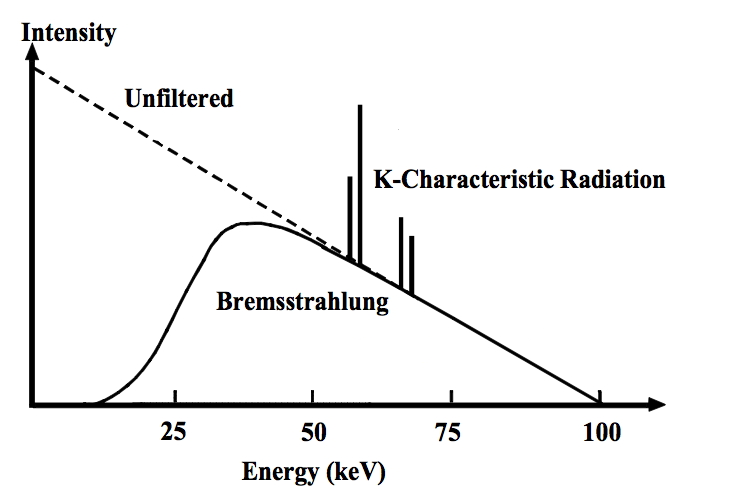
\includegraphics[width=0.9\textwidth]{illustrations/XrtSpectrum_edit.png}
  \caption[Röntgenspektrum charakteristisch und kontinuierlich]{Abgebildet ist ein typisches Röntgenspektrum, bestehend einerseits aus den charakteristischen Peaks der Schalenübergänge und andererseits aus einem kontinuierlichen Bremsspektrum. Das Abflachen im niederenergetischen Bereich wird durch Wechselwirkung der Photonen mit Materie bedingt, im Vakuum gibt es daher kein Abflachen (gestrichelt) \cite[bearbeitet]{spectrum}.}
  \label{fig:spectrumXray}
\end{figure}

